\documentclass{beamer}
\usepackage[right]{eurosym}
\usepackage{latexsym}
\usepackage{pgf,pgfarrows,pgfnodes,pgfautomata,pgfheaps}
\usepackage{color}
\usepackage{bbm}
\usepackage[english]{babel}
\usepackage[utf8]{inputenc}
% \usepackage[vmargin=25mm, top=20mm, bottom=25mm, left=28mm, right=28mm, includehead]{geometry}
% \usepackage{parskip}
\usepackage{csquotes}
\usepackage{german}
\usepackage{ngerman}
\usepackage{microtype}
\usepackage{amsfonts}
\usepackage{amssymb}
\usepackage{amsmath}
\usepackage{graphicx}
\usepackage{extarrows}
\usepackage{amsthm}
\usepackage{bookmark}
\usepackage{mathrsfs}
\usepackage{scrextend}
\usepackage{tikz}
\usepackage{subcaption}
\usepackage{float}
\usepackage{wrapfig}
\usepackage[singlelinecheck=false,justification=justified]{caption}
\usepackage[ruled,vlined]{algorithm2e}
\usepackage{algpseudocode}
\usepackage{mathtools}
\usepackage{hyperref}
\usepackage{graphicx}
\usepackage{times}
\usepackage[T1]{fontenc}


\graphicspath{{./graphics/}}

\usepackage[
    left = \flqq{},%
    right = \frqq{},%
    leftsub = \flq{},%
    rightsub = \frq{} %
]{dirtytalk}


\bibliographystyle{acm}

\newcommand{\uz}{\wegde}
\newcommand{\oz}{\vee}
\newcommand*\xor{\mathbin{\oplus}}
\everymath{\displaystyle}
\newcommand{\N}{\mathbb{N}}
\newcommand{\Prob}{\mathbb{P}}
\newcommand{\Z}{\mathbb{Z}}
\newcommand{\R}{\mathbb{R}}
\newcommand{\Q}{\mathbb{Q}}
\newcommand{\C}{\mathbb{C}}
\newcommand{\source}[1]{\caption*{Source: {#1}} }
\captionsetup[figure]{font=footnotesize}
\usepackage{commath}
\usepackage{esdiff}
\DeclareMathOperator{\Var}{\mathbf{Var}}
\DeclareMathOperator{\EW}{\mathbf{E}}
\DeclareMathOperator{\WS}{\mathbf{P}}
\DeclareMathOperator{\Cov}{\mathbf{Cov}}
\newcommand{\notimplies}{\;\not\!\!\!\implies}

% Set up

\mode<presentation>
{
  \usetheme{Warsaw}
  \setbeamercovered{transparent}
}
% Oder was auch immer. Zu beachten ist, das Font und Encoding passen
% m�ssen. Falls T1 nicht funktioniert, kann man versuchen, die Zeile
% mit fontenc zu l�schen.

\title[]{TC-VAE: Uncovering Out of distribution generative factors}
\author{Andreas Loehr}
\institute{Goethe Universität Frankfurt a.M.}
\date{
  \vspace{0.2cm}
  Seminar Pattern Analysis and Machine Intelligence
  \vspace{0.4cm}
  \newline 06/22/2023\\
  \vspace{0.3cm} % 0.4cm
  }
\subject{Informatik}

\let\definition\relax
\let\theorem\relax
% \let\theorem\relax
\theoremstyle{definition}
\newtheorem{definition}[section]{Definition}
% \newtheorem{definition_theorem}[definition]{Definition und Satz}

\newtheorem{cus_theorem}[section]{Satz}
%\newtheorem{def_theorem}[section]{Definition und Satz}
% \newtheorem{lemma}[definition]{Lemma}
% \newtheorem{remark}[definition]{Bemerkung}
% \newtheorem{remark_ex}[definition]{Beispiel}
% \newtheorem{notation}[definition]{Notation}
\newtheorem{remark}{Bemerkung}
\begin{document}
  \AtBeginSection[]
  {
      \begin{frame}
          \tableofcontents[currentsection]
      \end{frame}
    }
    % title page
  \begin{frame}
    \begin{titlepage}
    \end{titlepage}
  \end{frame}
  \begin{frame}
    \frametitle{Structure of the presentation (info sheet)}
    \begin{itemize}
      \item background/ preliminary work
      \item approach
      \item results
      \item discussion and conclusion
    \end{itemize}
  \end{frame}
  %intro to generative modelling. The problem statement
  \section{Representation Learning and Generative Modeling}
    \begin{frame}
      \frametitle{The Problem statement}
      \begin{itemize}
        \item Problem: Given data $X \in \mathbb{R}^{d}$ find a \textit{good} latent representation $Z \in \mathbb{R}^{m}$, $d, m \in \mathbb{N}$
        \item Example: $X$ images of fruit, $Z$ latent representation representing shape, texture, color etc.
        \end{itemize}
      \end{frame}

      \begin{frame}
        \frametitle{Definitions and Notation}
        \begin{itemize}
          \item \textbf{Data Generative Factors:} True underlying factors / attributes of the data
          \item \textbf{Latent Variable:} 1 dimensional variable
          \item \textbf{Latent Representation:} The vector of latent variables
        \end{itemize}
      \end{frame}

    \begin{frame}
      \frametitle{What is a good learned latent representation?}
      \begin{itemize}
        \item captures the true generative factors of the dataset
        \item interpretable
              $\rightarrow$ Optimally, single component of latent representation represents single generative factor
        \item sufficiently informative (captures majority of data generative factors)
        \item balanced
        \item Regularity
        \item TODO: completeness definition
        %, i.e. generative factors underrepresented in training data still have correspoding latent factor factors underrepresented in training data still have correspoding latent factor factors underrepresented in training data still have correspoding latent factor
        % in the sense that even generative factors which are underrepresented in the dataset do have a correspoding latent factor
      \end{itemize}
    \end{frame}

    \begin{frame}
        \frametitle{Why bother to learn good representations?}
        \begin{itemize}
          \item Facilitate downstream tasks like classification
          \item Generative modeling: control generative factors explictly by tweaking the corresponding latent variables
          % TODO: add more reasons and illustrate
        \end{itemize}
      \end{frame}

    \section{(Variational) Autoencoders}
    \begin{frame}
      \frametitle{Means to learn latent representations}
      \begin{itemize}
        \item Principal component analysis (PCA)? $\rightarrow$ Lack of interpretability
        \item (Regular) Autoencoders? $\rightarrow$ Lack of regularity
        % explain regularity - refer to Medium article/ paper
        % https://towardsdatascience.com/understanding-variational-autoencoders-vaes-f70510919f73
        \item Variational Autoencoders (VAE)?
      \end{itemize}
    \end{frame}

    \begin{frame}
      \frametitle{Autoencoders}
      % source autoencoder illustration
      %https://miro.medium.com/v2/resize:fit:4266/1*QEmCZtruuWwtEOUzew2D4A.png
      %\begin{center}
      \begin{figure}
        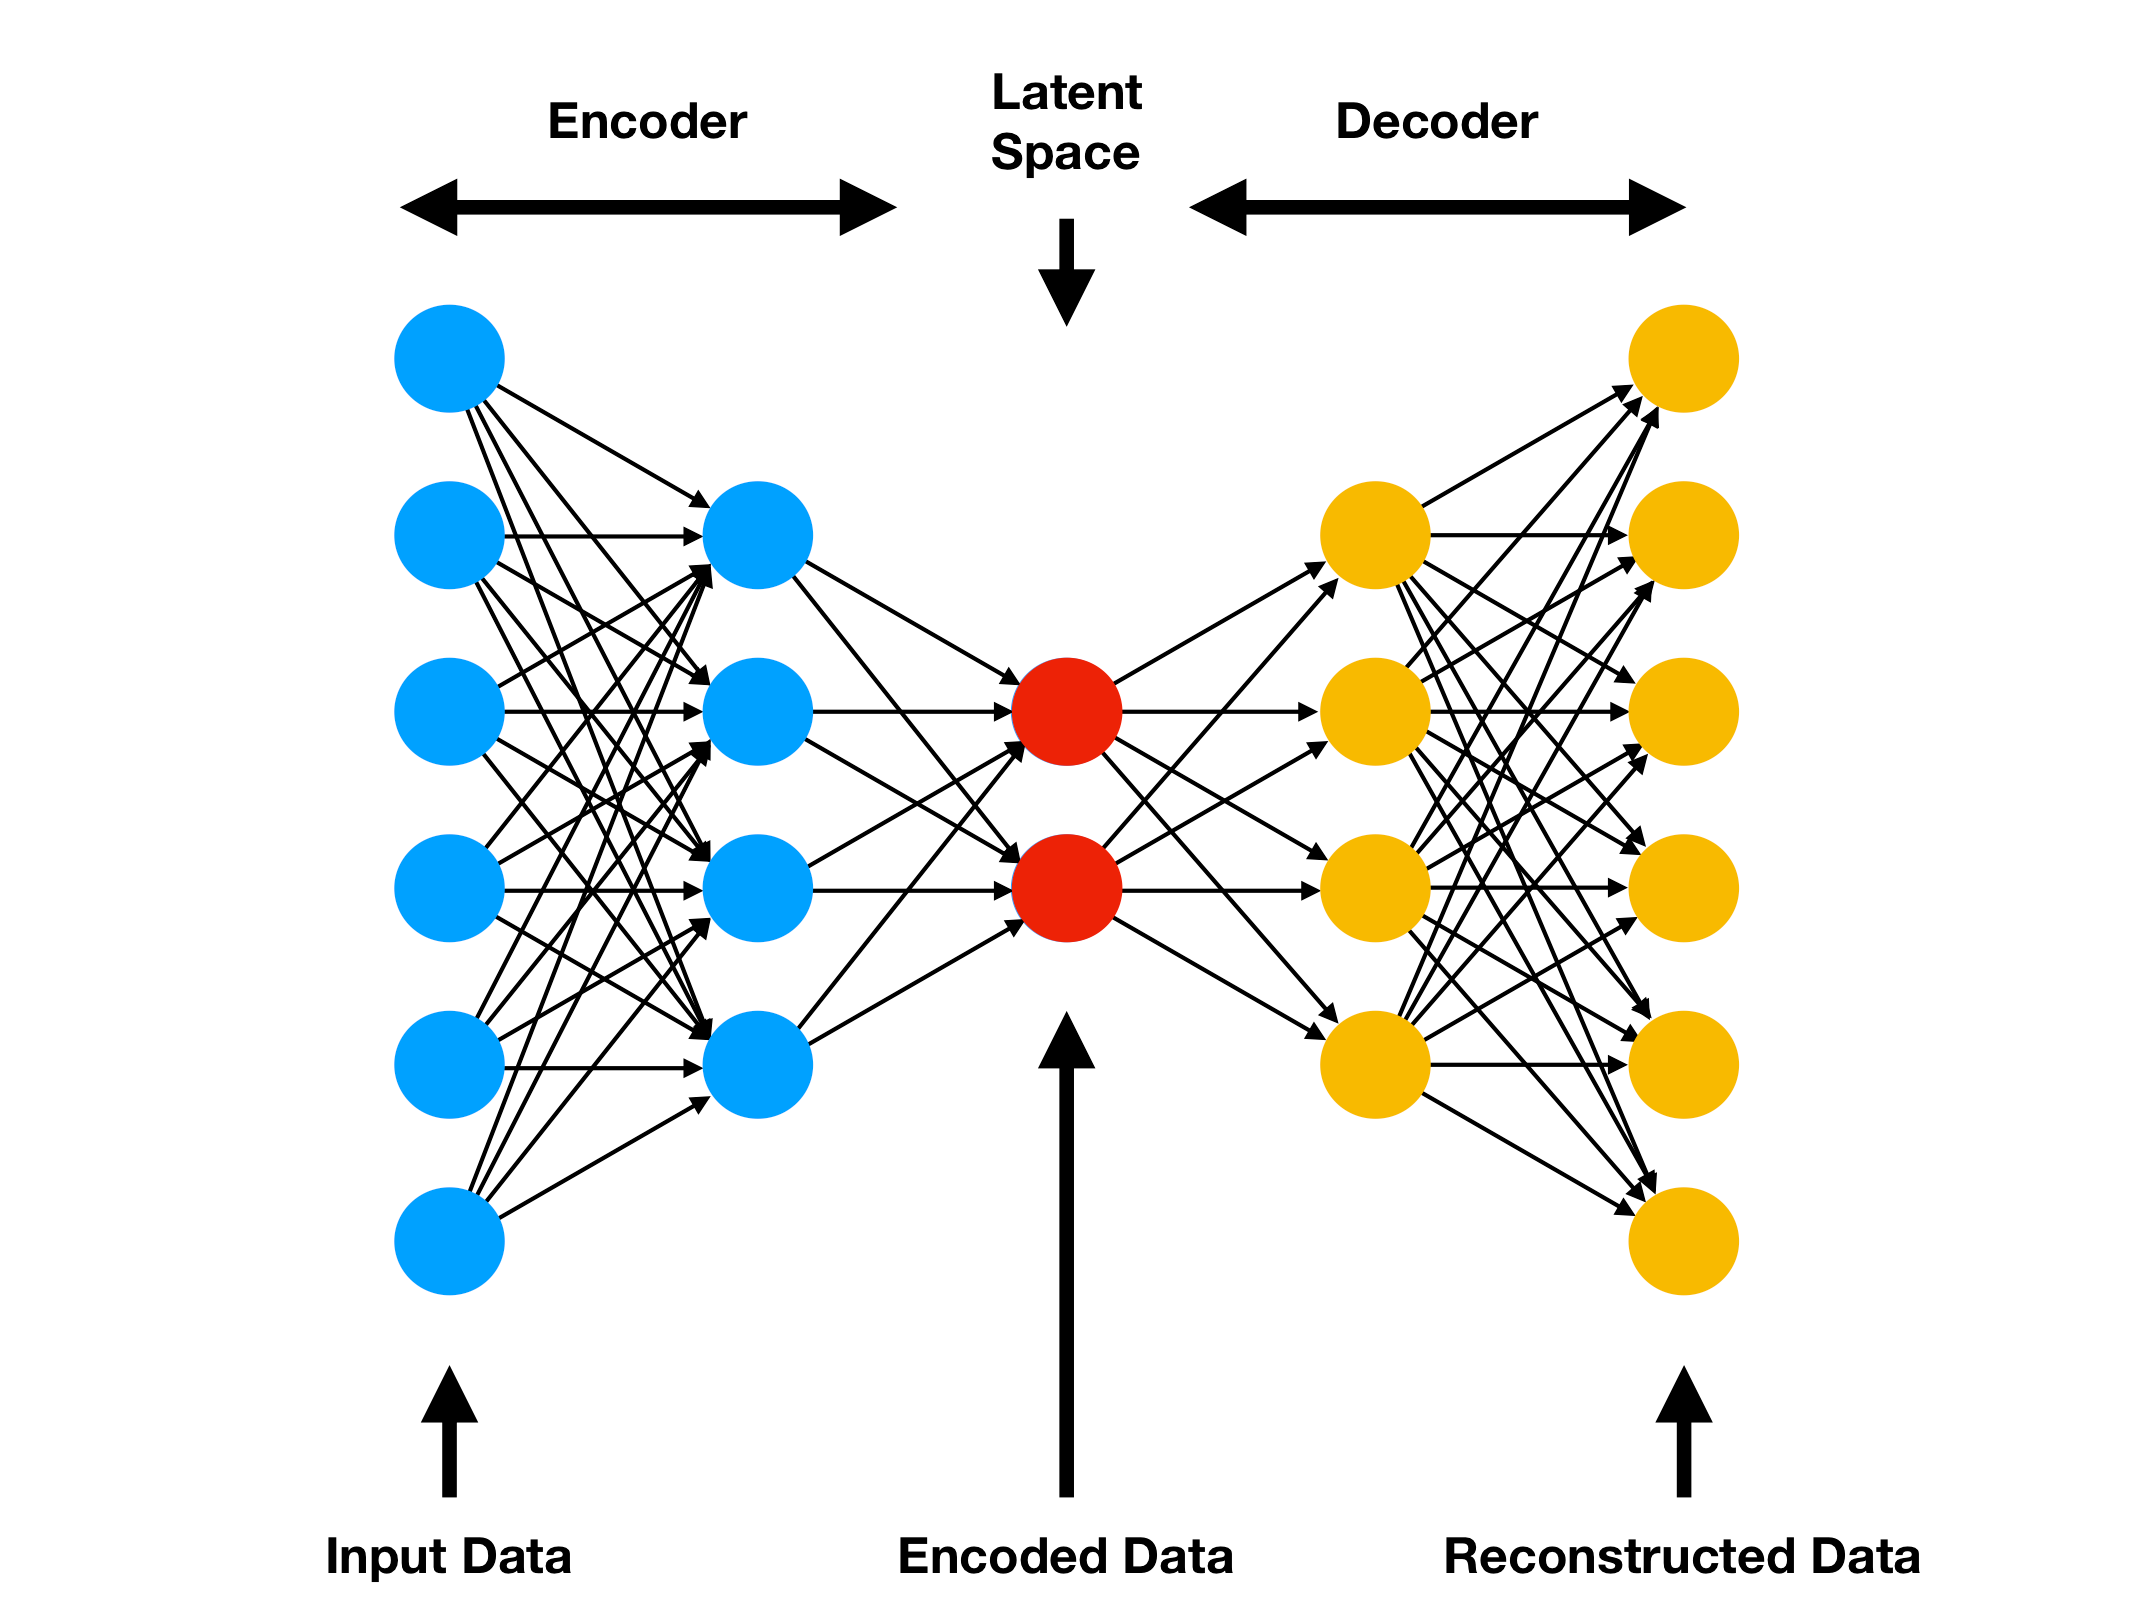
\includegraphics[scale= 0.09]{Autoencoder_illustration.png}
        \caption*{Source: https://medium.com/autoencoder-for-anomaly-detection/autoencoder-for-anomaly-detection-db6178ad07b2}
        % explain graphics quickly
      \end{figure}
      % \end{center}

    \end{frame}
    \begin{frame}
      \frametitle{Variational Autoencoders}
      \begin{figure}
        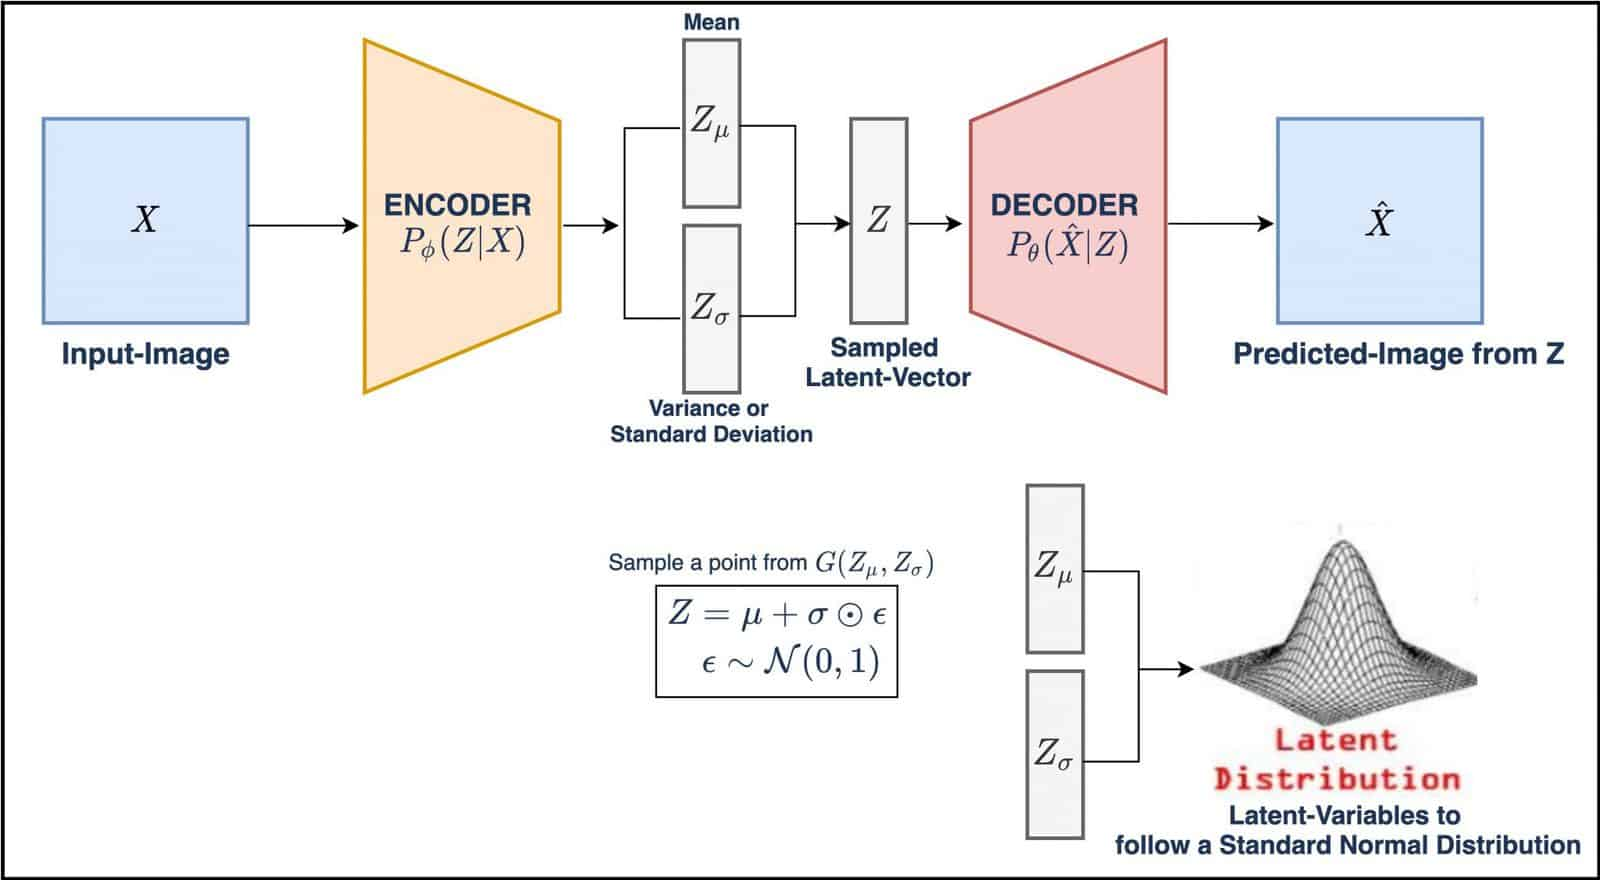
\includegraphics[scale=.125]{vae-diagram.jpg}
        \caption{Source: TODO}
      \end{figure}
      \vspace{-5mm}
      \begin{itemize}
        \item Generative model consisting of probabilisitic encoder and decoder
        \item Encoder \& decoder parametrize probability distributions over latent space and data respectively
      \end{itemize}
      % explain the graphics

    \end{frame}
    \begin{frame}
      \frametitle{Training Variational Autoencoders}
      Inspecting Encoder and Decoder
      The variational lower bound (ELBO)
    \end{frame}

    \begin{frame}
      \frametitle{Shortcomings}
    \end{frame}

    \begin{frame}
      \frametitle{Trying to Fix VAEs}
      $\beta$-VAEs and alternatives
    \end{frame}


  \section{TC-VAEs}

    \begin{frame}
      \frametitle{Shannon Entropy}
      TODO: Definition and Intuition of Shannon Entropy
    \end{frame}

    \begin{frame}
      \frametitle{mutual information}
      TODO: Definition and intuition of mutual information
    \end{frame}

    \begin{frame}
      \frametitle{Information Bottleneck and Deep Variational IB}
      TODO: Definition and Intuition
    \end{frame}

    \begin{frame}
      \frametitle{Total Correlation}
      TODO: Total correlation def and intuition
    \end{frame}

    \begin{frame}
      \frametitle{A new objective}
      Using TC as an objective
      Combination of different terms promoting different behavior
      Explanation of the single terms, given an intuition
    \end{frame}

    \begin{frame}
      \frametitle{A convex lower bound}
      Presenting the TC convex lower bound actually used in optimization
    \end{frame}


  \section{Experiments and Results}
    \begin{frame}
      \frametitle{Experiment Design}
      \begin{itemize}
        \item datasets + image of data to illustrate
        \item baseline models
        \item evaluation methods (i.e. downstream scores, qualitative (visual))
      \end{itemize}
    \end{frame}

    \begin{frame}
      \frametitle{Results}
      \begin{itemize}
        \item Qualitative: Traversals through latent space and discovery of 2 OOD generative factors (include picture)
        \item Quantitative: on datasets using abovementionEd metrics.
        \item Stress the performance on unbalanced datasets
      \end{itemize}
    \end{frame}

  \section{Discussion and Conclusion}
    \begin{frame}
      \frametitle{Discussion and Conclusion}
      \begin{itemize}
        \item Inspiration from Multiview representation learning (OOD generative factors correspond to missing views)
        \item Uncovering OOD generative factors $\equiv$ inferring missing views
        \item Experimental validation that TC-VAE is capable of uncovering OOD generative factors
        \item missing view also problematic for downstream tasks. underrepresented views may be seen as outliers
        \item main shortcoming: Terms appearing as part of the bound do promote conflicting behavior during minization
        \item unbalanced generative factors in dataset $\implies$ disentanglement deteriorates.
      \end{itemize}
    \end{frame}
\end{document}
